\documentclass[conference]{IEEEtran}

\usepackage[T1]{fontenc}
\usepackage[utf8]{inputenc}
\usepackage{listings}
\usepackage{todonotes}
\usepackage[nocompress]{cite}

\usepackage{algorithm}
\usepackage{algpseudocode}
\usepackage{hyperref}
\usepackage{amsmath}
\usepackage{amssymb}
\usepackage{amsthm}
\usepackage{amsfonts}
\usepackage{mathpartir}
\usepackage{subcaption}

\usepackage{tikz}
\usetikzlibrary{arrows}

\newcommand{\ottifc}{Ott-IFC}
\newcommand{\config}[3]{\ensuremath{\langle #1, #2, #3 \rangle}}
\newcommand{\emits}[3]{\ensuremath{#2\downarrow_{#1}#3}}
\newcommand{\proj}[2]{\ensuremath{{#1 \! \upharpoonright  \! {#2}}}}
\newcommand{\step}{{\ensuremath{\Downarrow}}}

\definecolor{grey}{rgb}{0.8,0.8,0.8}
\definecolor{code-background}{RGB}{255, 248, 220}
\definecolor{code-comment}{RGB}{196, 42, 42}
\definecolor{code-linenumber}{rgb}{0.5,0.5,0.5}
\definecolor{code-keyword}{RGB}{148, 0, 211}
\definecolor{coqatoo-pink}      {RGB}{255, 107, 104}
\definecolor{coqatoo-gray}      {RGB}{64, 64, 64}
\definecolor{coqatoo-yellow}    {RGB}{239, 223, 0}
\lstset{
   backgroundcolor=\color{code-background},   	% choose the background color; you must add \usepackage{color} or \usepackage{xcolor}
   basicstyle=\tt\footnotesize,       			% the size of the fonts that are used for the code
   breakatwhitespace=false,         			% sets if automatic breaks should only happen at whitespace
   breaklines=true,                 			% sets automatic line breaking
   captionpos=none,                    			% sets the caption-position to bottom
   commentstyle=\color{code-comment},   		% comment style
   deletekeywords={...},            			% if you want to delete keywords from the given language
   escapeinside={\%*}{*)},          			% if you want to add LaTeX within your code
   extendedchars=true,              			% lets you use non-ASCII characters; for 8-bits encodings only, does not work with UTF-8
   frame=tb,
   framerule=0pt,
   framextopmargin=0pt,
   framexbottommargin=0pt,
   keepspaces=true,                 			% keeps spaces in text, useful for keeping indentation of code (possibly needs columns=flexible)
   keywordstyle=\color{code-keyword},       						% keyword style
   language=ML,                 				% the language of the code
   morekeywords={Lemma, Proof, Qed, if, then, else, end, skip, stop, read, from, write, to},            % if you want to add more keywords to the set
   numbers=none,                    			% where to put the line-numbers; possible values are (none, left, right)
   numbersep=5pt,	                   			% how far the line-numbers are from the code
   numberstyle=\tiny\color{code-linenumber}, 	% the style that is used for the line-numbers
   rulecolor=\color{black}, 	        		% if not set, the frame-color may be changed on line-breaks within not-black text (e.g. comments (green here))
   showspaces=false,            	    		% show spaces everywhere adding particular underscores; it overrides 'showstringspaces'
   showstringspaces=false,          			% underline spaces within strings only
   showtabs=false,                  			% show tabs within strings adding particular underscores
   stepnumber=1,                    			% the step between two line-numbers. If it's 1, each line will be numbered
   stringstyle=\color{black},            		% string literal style
   tabsize=2,                       			% sets default tabsize to 2 spaces
   gobble=0,									% number of characters to remove at the beginning of each line
   mathescape=true,								% to render math symbols in the listing (between $)
   title=\lstname,                   			% show the filename of files included with \lstinputlisting; also try caption instead of title
   belowcaptionskip = 0cm
}

\begin{document}

\title{Ott-IFC: Automatically Generating Information-Flow Control Mechanism Specifications}

%\author{
%	\IEEEauthorblockN{Andrew Bedford}
%	\IEEEauthorblockA{Laval University\\
%		Quebec, Canada\\
%		andrew.bedford.1@ulaval.ca}
%}

\maketitle

% Abstract
\begin{abstract}
	Developing information-flow control mechanisms can be a difficult and time-consuming task due to the numerous and subtle ways through which information may flow in a program, particularly when dealing with complex programming languages. 
	
	In order to make this task easier, we present in this paper a tool called \emph{\ottifc} that can automatically generate information-flow control mechanism specifications (e.g., semantics of a runtime monitor) from programming language specifications (i.e., syntax and semantics).
\end{abstract}

\begin{IEEEkeywords}
	language-based security; information-flow control; development tool
\end{IEEEkeywords}

\section{Introduction}
Modern operating systems rely mostly on access-control mechanisms to protect users information. However, access control mechanisms are insufficient as they cannot regulate the propagation of information once it has been released for processing. To address this issue, a new research trend called \emph{language-based information-flow security}~\cite{DBLP:journals/jsac/SabelfeldM03} has emerged. The idea is to use techniques from programming languages, such as program analysis, monitoring, rewriting and type checking, to enforce information-flow policies (e.g., information from a private file should not be saved in a public file). Mechanisms that enforce such policies (e.g., \cite{DBLP:journals/jcs/VolpanoIS96, DBLP:conf/csfw/ChudnovN10,DBLP:conf/csfw/AskarovCM15,DBLP:journals/compsec/BedfordCDKT17}) are called \emph{information-flow control mechanisms}. 

Most information-flow control mechanisms seek to enforce a policy called \emph{non-interference}~\cite{DBLP:conf/sp/GoguenM82a}, which essentially states that private information may not interfere with the publicly observable behavior of a program. To enforce non-interference, a mechanism must take into account two types of information flows: \emph{explicit flows} and \emph{implicit flows}~\cite{DBLP:journals/cacm/Denning76}.

An insecure explicit information flow occurs when private information influences public information through a data dependency. For example in Listing~\ref{listing:explicit-flow}, the value that is written to \lstinline{publicFile} depends on the value of \lstinline{x}, which in turn depends on the value of \lstinline{privateValue}. Hence, any output of \lstinline{x} will reveal something about \lstinline{privateValue}.
\begin{lstlisting}[captionpos=b, caption=Insecure explicit flow, label=listing:explicit-flow]
  x := privateValue + 42;
  write x to publicFile
\end{lstlisting}
Explicit flows can be prevented by associating labels to sensitive information and propagating them whenever the information is used; a process known as \emph{tainting}.

\pagebreak
An insecure implicit information flow occurs when private information influences public information through the control-flow of the application. For example in Listing~\ref{listing:implicit-flow}, the value that is written to \lstinline{publicFile} depends on the condition \lstinline{privateValue > 0}. 
%Because of this, someone observing the content of \lstinline{publicChannel} could learn whether or not \lstinline{privateValue} is greater than zero.

\begin{lstlisting}[captionpos=b, caption=Insecure implicit flow, label=listing:implicit-flow]
  if (privateValue > 0) then
    write 0 to publicFile
  else
    write 1 to publicFile
  end
\end{lstlisting}
Implicit flows can be prevented using a \emph{program counter}, which keeps track of the context in which a command is executed.

While techniques to prevent insecure explicit and implicit flows are well-known and widely used~\cite{DBLP:journals/jsac/SabelfeldM03}, they are, to the best of our knowledge, still being applied manually when designing information-flow control mechanisms. This can lead to errors, failed proof attempts and time wasted. In order to make this task less laborious and reduce the risk of errors, we present in this paper a tool called \ottifc\ that can, given a programming language's specification (i.e., syntax and semantics), automatically apply those techniques and generate information-flow control mechanism specifications.

\subsubsection*{Contributions}
\begin{itemize}
	\item We present \ottifc\ and illustrate its use on a simple imperative language (Section~\ref{section:ott-ifc}).
	\item We provide rough sketches of the proofs that show that the generated mechanisms are sound and do not change the semantics of the executed programs (Section~\ref{section:soundness}).
\end{itemize}

%Approach and Uniqueness: Describe your approach in attacking the problem and clearly state how your approach is novel.
\section{Overview of Ott-IFC}\label{section:ott-ifc}
As the name implies, the specifications that \ottifc\ takes as input (and outputs) are written in Ott~\cite{DBLP:journals/jfp/SewellNOPRSS10, Ott}. Ott is a tool that can generate LaTeX, Coq~\cite{Coq} or Isabelle/HOL~\cite{IsabelleHOL} versions of a programming language's specification. The specification is written in a concise and readable ASCII notation that resembles what one would write in informal mathematics (see the Listings of Section~\ref{section:ott-ifc}).

Hence, the development process of a mechanism using Ott and \ottifc\ would look like this:
\begin{enumerate}
  \item Write specification of the language on which we want to enforce non-interference in Ott.
  \item Use \ottifc\ to generate the mechanism's specification.
  \item Use Ott to export the mechanism's specification to LaTeX, Coq or Isabelle/HOL and complete the implementation.
\end{enumerate}

For the moment, \ottifc\ requires that the language specification follows a certain format. Namely, we require:
\begin{itemize}
	\item[\textbf{R1}] that it uses either small-step or big-step operational semantics;
	\item[\textbf{R2}] that the program configurations be of the form $\langle \textit{c}, \textit{m}, \textit{o}\rangle$, where $c$ is the command to be evaluated, $m$ is the current memory and $o$ is the current output trace;
	\item[\textbf{R3}] that the outputs be appended to the output trace using the notation $o\!::\!(\textit{channel},\, \textit{value})$, where $\textit{value}$ represents the output's value and $\textit{channel}$ its location;
	\item[\textbf{R4}] that the syntax be composed of \emph{commands}, which may read/write the memory or produce outputs, and \emph{expressions}, which may only read the memory;
	\item[\textbf{R5}] that the semantics preconditions don't include calls to functions which may have side-effects and that they 
\end{itemize}
These requirements mean that \ottifc\ won't work with most functional languages; only imperative languages are supported. This is because in functional languages, the distinction between commands and expressions is less apparent and sometimes inexistent. Note that this is not a technical limitation, but rather a choice that we made in order to simplify the approach. 

%\subsection{Rewriting Algorithm}
%\begin{algorithm}
%	\caption{\ottifc's rewriting algorithm pseudo-code}
%	\label{algorithm:rewriting}
%	\begin{algorithmic}[1]
%		\Procedure{GenMonitor}{$\textit{syntax}, \textit{semantics}$}
%		\State Verify that the specification is supported
%		\State Identify expression and command non-terminals
%		\For{\textbf{each} \textit{command} \textbf{in} \textit{syntax}}{}
%		\State Identify rules for \textit{command} in \textit{semantics}
%		\State Build graphs
%			\For{\textbf{each} \textit{rule}}{}
%				\If {\textit{rule} or one of its successor in the graph modifies the memory}{}
%				\State Update the modified variable's label
%				\EndIf
%				\If {\textit{rule} or one of its successor in the graph produces an output}{}
%					\State Insert guard condition
%				\EndIf
%				\If {\textit{command} may affect the control-flow of the application}{}
%				\State Update the pc
%				\State Update the label of variables that could be modified
%				\EndIf
%			\EndFor
%		\EndFor
%		\EndProcedure
%	\end{algorithmic}
%\end{algorithm}

%\subsection{Example}
An example of a language that satisfies these requirements is the imperative language whose syntax is defined in Listing~\ref{listing:input-syntax} and semantics in Listings~\ref{listing:input-semantics-arithmetic}, \ref{listing:input-semantics-booleans} and \ref{listing:input-semantics-commands}.

\begin{lstlisting}[label=listing:input-syntax,captionpos=b,caption=Ott syntax of a simple imperative language]
  arith_expr, a ::= x | n | a1 + a2 | a1 * a2 
  bool_expr, b ::= true | false | a1 < a2
  commands, c ::= stop | skip | x := a | c1 ; c2 | 
                  read x from ch | write x to ch |
                  if b then c1 else c2 end | 
                  while b do c end

\end{lstlisting}

\begin{lstlisting}[label=listing:input-semantics-arithmetic,captionpos=b,caption=Ott small-step semantics of arithmetic expressions]
	%%% Variable %%%
	m(x) = n
	---------------------------------------- :: lookup
	<x, m, o> --> <n, m, o>

	%%% Constant %%%
	---------------------------------- :: int_constant
	<n, m, o> --> <n, m, o>
	
	%%% Addition %%%
	<a1, m, o> --> <a1', m, o>
	--------------------------------- :: add_aexp_aexp
	<a1 + a2, m, o> --> <a1' + a2, m, o>
	
	<a2, m, o> --> <a2', m, o>
	---------------------------------- :: add_int_aexp
	<n1 + a2, m, o> --> <n1 + n2, m, o>
	
	n1 + n2 = n3
	----------------------------------- :: add_int_int
	<n1 + n2, m, o> --> <n3, m, o>
	
	%%% Multiplication %%%
	<a1, m, o> --> <a1', m, o>
	-------------------------------- :: mult_aexp_aexp
	<a1 * a2, m, o> --> <a1' * a2, m, o>
	
	<a2, m, o> --> <a2', m, o>
	--------------------------------- :: mult_int_aexp
	<n1 * a2, m, o> --> <n1 * n2, m, o>
	
	n1 * n2 = n3
	---------------------------------- :: mult_int_int
	<n1 * n2, m, o> --> <n3, m, o>
\end{lstlisting}

\begin{lstlisting}[label=listing:input-semantics-booleans,captionpos=b,caption=Ott small-step semantics of boolean expressions]
	%%% Lower Than %%%
	<a1, m, o> --> <a1', m, o>
	---------------------------------- :: lt_aexp_aexp
	<a1 < a2, m, o> --> <a1' < a2, m, o>
	
	<a2, m, o> --> <a2', m, o>
	----------------------------------- :: lt_int_aexp
	<n1 < a2, m, o> --> <n1 < n2, m, o>
	
	n1 < n2 = true
	------------------------------- :: lt_int_int_true
	<n1 < n2, m, o> --> <true, m, o>
	
	n1 < n2 = false
	------------------------------ :: lt_int_int_false
	<n1 < n2, m, o> --> <false, m, o>
\end{lstlisting}

\begin{lstlisting}[label=listing:input-semantics-commands,captionpos=b,caption=Ott small-step semantics of commands]
	%%% Skip %%%
	------------------------------------------ :: skip
	<skip, m, o> --> <stop, m, o>

	%%% Assignment %%%
	<a, m, o> --> <a', m, o>
	----------------------------------- :: assign_aexp
	<x := a, m, o> --> <x := a', m, o>
	
	------------------------------------ :: assign_int
	<x := n, m, o> --> <stop, m[x |-> n], o>
	
	%%% Sequence %%%
	<c1, m, o> --> <c1', m', o'>
	------------------------------------------ :: seq1
	<c1 ; c2, m, o> --> <c1' ; c2, m', o'>
	
	------------------------------------------ :: seq2
	<skip ; c2, m, o> --> <c2, m, o>
	
	%%% Read %%%
	m(ch) = n
	------------------------------------------ :: read
	<read x from ch, m, o> --> <stop, m[x |-> n], o>
	
	%%% Write %%%
	m(x) = n
	----------------------------------------- :: write
	<write x to ch, m, o> --> 
	<stop, m[ch |-> n], o::(ch, n)>
	
	%%% If %%%
	<b, m, o> --> <b', m, o>
	--------------------------------------- :: if_eval
	<if b then c1 else c2 end, m, o> --> 
	<if b' then c1 else c2 end, m, o>
	
	--------------------------------------- :: if_true
	<if true then c1 else c2 end, m, o> --> 
	<c1, m, o>
	
	-------------------------------------- :: if_false
	<if false then c1 else c2 end, m, o> --> 
	<c2, m, o>
	
	%%% While %%%
	----------------------------------------- :: while
	<while b do c end, m, o> --> 
	<if b then c;while b do c end else skip end, m, o>
\end{lstlisting}

To illustrate how our approach works, we will generate an information-flow control mechanism (a runtime monitor) from this specification. Our approach can be decomposed into three steps: identifying commands and expressions, constructing evaluation-order graphs, rewriting the semantics.

\subsection{Step 1: Identifying commands and expressions}
To identify which non-terminals (e.g., \lstinline{a}, \lstinline{b}, \lstinline{c}) of the syntax correspond to commands and which correspond to expressions, we need to identify the semantics rule associated to each non-terminal. To do so, we analyze each rule of the syntax and generate a set of strings that represents their possible values. For example, for the non-terminal \lstinline{bool_expr} (a.k.a. \lstinline{b}), it would return the set of strings \{\lstinline{true, false, a < a, x < a, a < x, n < a, a < n, a + a < a, ...}\}. This set of string doesn't need to be exhaustive, only sufficiently so to be able to identify their use in the semantics. 

Using this set of strings, we can then detect the rules associated to the non-terminals by looking that the first element of the initial state configurations. In the case of \lstinline{bool_expr}, it would return the rules of Listing~\ref{listing:input-semantics-booleans}. Since none of these rules modify the memory or produce outputs, we can conclude that the non-terminals \lstinline{bool_expr} and \lstinline{b} are expressions.

Using the same reasoning, we can conclude that:
\begin{itemize}
	\item the expression non-terminals are \lstinline{arith_expr}, \lstinline{a}, \lstinline{bool_expr}, \lstinline{b}, \lstinline{x}, \lstinline{n}, and that the rules associated to those are the ones in Listings~\ref{listing:input-semantics-arithmetic} and \ref{listing:input-semantics-booleans};
	\item the commands non-terminals are \lstinline{commands, c}, and that the rules associates to those are the ones in Listing~\ref{listing:input-semantics-commands}.
\end{itemize}

\subsection{Step 2: Constructing evaluation-order graphs}
The next step consists in constructing \emph{evaluation-order graphs} for each command. These graphs represent the order in which the semantics rules may be evaluated for a specific command (see Figure~\ref{figure:evaluation-order-graphs}).
\begin{figure}[h]
\begin{subfigure}[t]{0.48\linewidth}
	\centering
	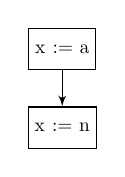
\begin{tikzpicture}
	\tikzset{vertex/.style = {shape=rectangle,draw,minimum height=0.75cm}}
	\tikzset{edge/.style = {->,> = latex'}}
	% vertices
	\node[vertex,scale=0.7] (assign1) at  (0,1) {\lstinline{x := a}};
	\node[vertex,scale=0.7] (assign2) at  (0,0) {\lstinline{x := n}};
	
	%edges
	\draw[edge] (assign1) to (assign2);
	\end{tikzpicture}
	\caption{Assign}
\end{subfigure}
~
\begin{subfigure}[t]{0.48\linewidth}
	\centering
	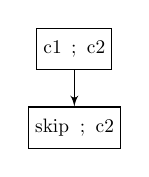
\begin{tikzpicture}
	\tikzset{vertex/.style = {shape=rectangle,draw,minimum height=0.75cm}}
	\tikzset{edge/.style = {->,> = latex'}}

	\node[vertex,scale=0.7] (seq1) at  (0,1) {\lstinline{c1 ; c2}};
	\node[vertex,scale=0.7] (seq2) at  (0,0) {\lstinline{skip ; c2}};
	\draw[edge] (seq1) to (seq2);
	\end{tikzpicture}
	\caption{Sequence}
\end{subfigure}

\begin{subfigure}{1\linewidth}
	\centering
	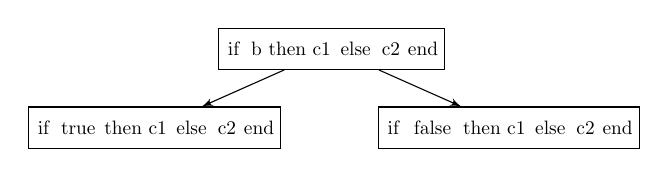
\begin{tikzpicture}
		\tikzset{vertex/.style = {shape=rectangle,draw,minimum height=0.75cm}}
		\tikzset{edge/.style = {->,> = latex'}}
		
		\node[vertex,scale=0.7] (if) at  (2.25,-1) {\lstinline{if b then c1 else c2 end}};
		\node[vertex,scale=0.7] (iftrue) at  (0,-2) {\lstinline{if true then c1 else c2 end}};
		\node[vertex,scale=0.7] (iffalse) at  (4.5,-2) {\lstinline{if false then c1 else c2 end}};
		
		\draw[edge] (if) to (iftrue);
		\draw[edge] (if) to (iffalse);
	\end{tikzpicture}
	\caption{Conditional}
\end{subfigure}
%	\center
%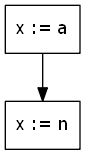
\includegraphics[width=0.33\linewidth]{images/graph-assign.png}~\\~\\
%\end{minipage}
%\begin{minipage}{0.49\linewidth}
%	\center
%	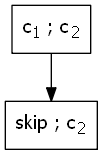
\includegraphics[width=0.4\linewidth]{images/graph-sequence.png}~\\~\\
%\end{minipage}
%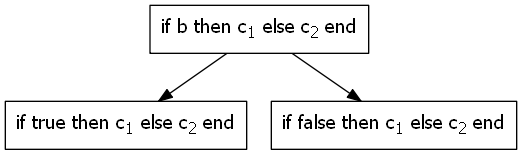
\includegraphics[width=\linewidth]{images/graph-if.png}
\caption{Evaluation-order graphs of the assign, sequence and conditional commands.}
\label{figure:evaluation-order-graphs}
\end{figure}

To construct these graphs, we use the set of strings produced in Step 1 to detect that the rules associated to the assign command are \lstinline{assign_aexp} and \lstinline{assign_int}, and that \lstinline{assign_aexp} will be evaluated first because \lstinline{x := a} is more general than \lstinline{x := n}. By more general, we mean that the set of strings that matches with \lstinline{x := a} also matches with \lstinline{x := n}, but the reverse is not true.

\subsection{Step 3: Rule-based rewriting}
The final step is to perform the actual rewriting of the semantics rules to insert a runtime monitor that enforces non-interference (i.e., a monitor that prevents insecure explicit and implicit flows of information). To do so, we try to replicate the thought process that a human would have when producing such a mechanism.

We start by inserting a program counter \lstinline{pc}, and a typing environment \lstinline{E}, which maps variables to their labels, in each command configurations. That is, configurations that have the form \lstinline{<c, m, o>} are changed to \lstinline{<c, m, o, pc, E>}.

To prevent explicit flows, we identify the commands that may modify the memory \lstinline{m} (e.g., the assign command). In their rules, we update the modified variable's label with the label of the expression variables that are used in the rule. If they also produce an output, then we insert a guard condition to ensure that no leak of information occurs.

To prevent implicit flows, we identify the commands that may influence the control-flow of the application using the evaluation-order graphs. That is, commands for which a program configuration may lead to two different program configurations (e.g., the if command). In other words, commands for which there are multiple "terminal nodes" (i.e., nodes that have no successors) in the evaluation-order graph. We then update the program counter \lstinline{pc} with the labels of the expression variables that are present in the rule.

So, for the language of our example, we would obtain the following rules (the changes are in {\color{red}red}):

\paragraph{Skip}
Because the \lstinline{skip} command does essentially nothing, it does not read/write the memory or produce outputs, the only change in the rule is the addition of the \lstinline{pc} and \lstinline{E} variables (line 2).
\begin{lstlisting}[label=listing:output-semantics-skip,numbers=right,captionpos=b,caption=Ott-IFC's output for the "skip" command]
	------------------------------------------ :: skip
	<skip, m, o, $\text{\color{red}pc, E}$> --> <stop, m, o, $\text{\color{red}pc, E}$>
\end{lstlisting}

\paragraph{Read}
The \lstinline{read} command reads the content of channel \lstinline{ch} and assigns its value to \lstinline{x}. For each expression variable found in the preconditions (i.e., \lstinline{ch, n}), we insert a label variable definition (lines 2 and 3). Note that \lstinline{|-} is the ASCII representation of $\vdash$ and \lstinline{|_|} of the supremum operator $\sqcup$. Since the memory is modified, we propagate the label of the expressions that influence the assigned variable's value (i.e., the ones used in the rule) and take into account the context in which the assignment occurs (line 6).
\begin{lstlisting}[label=listing:output-semantics-read,captionpos=b,numbers=right,caption=Ott-IFC's output for the "read" command]
	m(ch) = n
	$\text{\color{red}E |- ch : lch}$
	$\text{\color{red}E |- n : ln}$
	------------------------------------------ :: read
	<read x from ch, m, o, $\text{\color{red}pc, E}$> --> 
	<stop, m[x |-> n], o, $\text{\color{red}pc,}$ $\text{\color{red}E[x |-> pc |\_| lch |\_| ln]}$>
\end{lstlisting}

\paragraph{Write} The \lstinline{write} command writes the value of \lstinline{x} on the channel \lstinline{ch}. Because this command produces an output (i.e., it appends a value to \lstinline{o}), we add guard condition that ensures that no leak of information will occur at runtime (line 5). We do not update the label of the channel on which the output occurs even if it is modified because, if the execution is not stopped by the monitor, then it means that the channel's label is already greater than the label of the expression that is written.
\begin{lstlisting}[label=listing:output-semantics-write,numbers=left,captionpos=b,caption=Ott-IFC's output for the "write" command]
	m(x) = n
	$\text{\color{red}E |- x : lx}$
	$\text{\color{red}E |- n : ln}$
	$\text{\color{red}E |- ch : lch}$
	$\text{\color{red}lx |\_| ln |\_| pc <= lch}$
	----------------------------------------- :: write
	<write x to ch, m, o, $\text{\color{red}pc, E}$> --> 
	<stop, m[ch |-> n], o::(ch, n), $\text{\color{red}pc, E}$>
\end{lstlisting}

\paragraph{Assign}
While the \lstinline{assign_aexp} rule does not directly modify the memory, one of its successor in the evaluation-order graph (i.e., \lstinline{assign_int}) does. For this reason, we must update the label of the modified variable in, not only \lstinline{assign_int}, but also \lstinline{assign_aexp} (lines 6 and 12). This is to take into account the label of variables that are in the expression \lstinline{a} (before they disappear). This means that, in this case, the generated monitor won't allow the label of variables to be "downgraded" as a result of an assignment.
\begin{lstlisting}[label=listing:output-semantics-assign,numbers=left,captionpos=b,caption=Ott-IFC's output for the "assign" command]
	<a, m, o> --> <a', m, o>
	$\text{\color{red}E |- x : lx}$
	$\text{\color{red}E |- a : la}$
	----------------------------------- :: assign_aexp
	<x := a, m, o, $\text{\color{red}pc, E}$> --> 
	<x := a', m, o, $\text{\color{red}pc, E[x |-> lx |\_| pc |\_| la]}$>
	
	$\text{\color{red}E |- x : lx}$
	$\text{\color{red}E |- n : ln}$
	------------------------------------ :: assign_int
	<x := n, m, o, $\text{\color{red}pc, E}$> --> 
	<stop, m[x |-> n], o, $\text{\color{red}pc, E[x |-> lx |\_| pc |\_| ln]}$>
\end{lstlisting}

It may be interesting to note that, had the big-step version of the semantics been given to \ottifc\ instead, this would not be the case (see Listing~\ref{listing:output-semantics-assign-bigstep}). This is because in the big-step version, the assign command has only one rule. In other words, this means that the form of the specification given as input influences the permissiveness of the monitor that is returned by our tool (more on this in Section~\ref{section:discussion}).
\begin{lstlisting}[label=listing:output-semantics-assign-bigstep,captionpos=b,caption=Ott-IFC's output the big-step version of the "assign" command]
	<a, m, o> || <n, m, o>
	$\text{\color{red}E |- a : la}$
	---------------------------------------- :: assign
	<x := a, m, o, $\text{\color{red}pc, E}$> || 
	<stop, m[x |-> n], o, $\text{\color{red}pc, E[x |-> pc |\_| la]}$>
\end{lstlisting}



\paragraph{Sequence} The rules for the sequence do not modify the memory or produce outputs so, like the skip command, the only changes in the rules is the addition of the \lstinline{pc} and \lstinline{E} variables. Note however that we did not only update the configurations in the conclusion of the rule, but also in the precondition.
\begin{lstlisting}[label=listing:output-semantics-sequence,captionpos=b,caption=Ott-IFC's output for the "sequence" command]
	<c1, m, o, $\text{\color{red}pc, E}$> --> <c1', m', o', $\text{\color{red}pc, E'}$>
	------------------------------------------ :: seq1
	<c1 ; c2, m, o, $\text{\color{red}pc, E}$> --> 
	<c1' ; c2, m', o', $\text{\color{red}pc, E'}$>
	
	------------------------------------------ :: seq2
	<skip ; c2, m, o, $\text{\color{red}pc, E}$> --> <c2, m, o, $\text{\color{red}pc, E}$>
\end{lstlisting}



\paragraph{If}
In this language, the \lstinline{if} command is the only that can directly cause the control-flow of a program to branch-out. We can tell this by looking at its evaluation-order graph (Figure ~\ref{figure:evaluation-order-graphs}): there are two terminal nodes (i.e, the \lstinline{if true} and \lstinline{if false}). For this reason, we update the \lstinline{pc} variables with the labels of the expression variables that are present in the rule (i.e., only \lstinline{b} in this case). 

We also insert a call to a function called \lstinline{updateModifVars} which will have to be implemented by the user. What it does is that it identifies all the variables that could have been modified in either \lstinline{c1} or \lstinline{c2}, and update their labels with the label of \lstinline{b} (line 3). This is to ensure that the labels of the variables after executing the \lstinline{if} is always the same, no matter which branch that is taken during execution. Note that the command variables that are used in the rule (\lstinline{c1} and \lstinline{c2}) are detected the same way that expression variables are detected: using the set of strings generated in Step 1.
\begin{lstlisting}[label=listing:output-semantics-if,numbers=right,captionpos=b,caption=Ott-IFC's output for the "if" command]
	<b, m, o> --> <b', m, o>
	$\text{\color{red}E |- b : lb}$
	$\text{\color{red}E1 = updateModifVars(E, pc |\_| lb, \{c1,c2\})}$
	-------------------------------------- :: if_eval
	<if b then c1 else c2 end, m, o, $\text{\color{red}pc, E}$> --> 
	<if b' then c1 else c2 end, m, o, $\text{\color{red}pc |\_| lb, E1}$>
	
	-------------------------------------- :: if_true
	<if true then c1 else c2 end, m, o, $\text{\color{red}pc, E}$> --> 
	<c1, m, o, $\text{\color{red}pc, E}$>
	
	------------------------------------- :: if_false
	<if false then c1 else c2 end, m, o, $\text{\color{red}pc, E}$> --> 
	<c2, m, o, $\text{\color{red}pc, E}$>
\end{lstlisting}

\paragraph{While} Like the skip and sequence commands, the semantics rule of the while command does not modify the memory or the output trace, hence the only change is the addition of the \lstinline{pc} and \lstinline{E} variables to the configurations. Note that, while the \lstinline{pc} variable is not updated here with the label of the condition variable \lstinline{b}, it will be when the \lstinline{if} (present in the final configuration) is evaluated (line 3). 
\begin{lstlisting}[label=listing:output-semantics-while,numbers=right,captionpos=b,caption=Ott-IFC's output for the "while" command]
	--------------------------------------- :: while
	<while b do c end, m, o, $\text{\color{red}pc, E}$> --> 
	<if b then c ; while b do c end else skip end, m, o, $\text{\color{red}pc, E}$>
\end{lstlisting}

\pagebreak
\section{Soundness}\label{section:soundness}
We have tested and validated that our approach works on multiple language specifications. However, to be sure that it works for \emph{any} specification that meets our requirements, we must formally define non-interference and prove that the generated mechanisms are indeed sound. Before formally defining non-interference, we first need to introduce some helpful technical concepts.

For our purposes, we assume that the labels, which represent levels of information, are organized in a finite lattice ${(\mathcal{L},\sqsubseteq)}$ which contains at least two elements: $L$ for the bottom of the lattice (least important) and $H$ for the top of the lattice (most important), i.e. $\forall l \in \mathcal{L}, L \sqsubseteq l \wedge l  \sqsubseteq H$.

The \emph{projection of trace $o$ to label $\ell$}, written \proj{o}{\ell}, is its restriction  to output events whose channels' labels are less than or equal to $\ell$.  Formally,
\begin{align*}
\proj{\epsilon}{\ell}      & = \epsilon     \\
\proj{(o\!::\!(ch,v))}{\ell} & = \left \{   \begin{array}{ll}
\!(\proj{o}{\ell})\!::\!(ch,v)\!\! &  \text{ if }   \levelOfChan{ch}   \sqsubseteq \ell \\
\proj{o}{\ell}  &   \text{ otherwise}
\end{array} \right.
\end{align*}
where \levelOfChan{ch} denotes the label of channel $ch$ (typically specified by the administrator).

We write $\emits{ }{\config{c}{m}{\epsilon}}{o}$ if execution of configuration $\config{c}{m}{\epsilon}$
can produce trace $o$.

We say that two memories $m$ and $m'$ are $\ell$-equivalent if they agree on the content of variables  (including channel variables) whose labels are $\ell$ or lower.

\begin{definition}[Non-interference\footnote{Also known as termination-insensitive non-interference}]
A program $p$ satisfies non-interference if for any $\ell \in \mathcal{L}$, and for any two memories $m$ and $m'$ that are $\ell$-equivalent, and for any trace $o$ such that $\emits{}{\config{p}{m}{\epsilon}}{o} $, then there is some trace $o'$, such that $\emits{}{\config{p}{m'}{\epsilon}}{o'}$ and $\proj{o}{\ell}$ is a prefix of $\proj{o'}{\ell}$ (or vice versa).
\end{definition}

\begin{theorem}[Soundness of enforcement]
	Let $M$ be a monitor generated by \ottifc\ from a language specification $S$ that satisfies the requirements of Section~\ref{section:ott-ifc}, $m$ be a memory and $p$ be a program written in the language specified by $S$. The execution of $p$ under monitor $M$ and memory $m$, denoted $M(\langle p, m, \epsilon \rangle)$, will be non-interferent.
\end{theorem}
\begin{proof}[Sketch]
	The arguments for the proof are similar to the ones presented in Section~\ref{section:ott-ifc}. 
	
	We start by showing that, if the evaluation of a command may cause a branch in the execution, then it will have multiple terminal states in the command-evaluation order graph.

	To show that there can be no explicit or implicit flows, we then proceed by structural induction on the types of commands: commands whose evaluation may modify the memory, commands whose evaluation may produce an output, commands whose evaluation does neither.
	
	We show that there can be no explicit flows because, any time that a variable's value is changed in the memory, we update its label (the only exception being channels) and that for any output, there is a guard condition. 
	
	We then show that there can be no implicit flows because, any time a branch in the control-flow could occur, we update the \lstinline{pc} variable with the label of \emph{all} expression variables that could have influenced the decision. We also point out that the \lstinline{pc} variable is present every time that a label is updated and in every inserted guard conditions.
\end{proof}

We also show that the generated runtime monitor preserves the semantics of the original program. That is, a program $p$ executed under the monitor $M$ produces exactly the same output as $p$ as long as it is allowed to continue;  it may be stopped at some point to prevent a leak. 

\begin{theorem}[Semantics preservation]\label{th:semantic-preservation}
	Let $p$ be a program, $m$ a memory, and $o, o'$ output traces.
	Then
\begin{align*}
	&M(\langle p, m, \epsilon \rangle) \downarrow o \Rightarrow\  \emits{ }{\config{p}{m}{\epsilon}}{o} \\
	&(\emits{ }{\config{p}{m}{\epsilon}}{o}  \wedge M(\langle p, m, \epsilon \rangle) \downarrow o') \Rightarrow\
	o\preceq o' \vee   o'\preceq o\
	\label{}
\end{align*}
	where $o' \preceq o$ means that $o'$ is a prefix of $o$.
\end{theorem}
\begin{proof}[Sketch]
	The semantics generated by \ottifc\ are the essentially the same as the as the original semantics. The only difference being the additional variables in the configurations (\lstinline{pc} and \lstinline{E}), and the definitions of label variables and guard conditions in the preconditions. For this reason, the only non-trivial case is when we insert guard conditions to prevent commands that modify the output trace from leaking information.
	
	If this guard condition inserted is true, then the output will occur as it would have in the non-monitored execution of the program. If the guard condition fails, then the execution of the monitored program will be stopped, and hence, no more outputs will occur (the non-monitored execution could produce other outputs).
\end{proof}


\section{Discussion}\label{section:discussion}
As far as we know, we are the first ones to propose a way to generate information-flow control mechanism specifications from programming language specifications. Our implementation is available online\footnote{The link will be made available once the peer-review process is finished} and open-source. We expect that our tool will be particularly useful to researchers in language-based security that need to quickly develop mechanisms for complex languages. 

For the moment, our tool can only produce one kind of mechanism: runtime monitors. We chose to generate runtime monitors because they seemed the simplest to generate: they are simply modified versions of the semantics given as input. However, the same logic could be used to produce other types of mechanisms, such as type systems.

Note that the mechanisms generated by our approach may not always be as permissive as those designed by humans. For example, when we update the labels of modified variables, we update it using the labels of \emph{all} the expression variables found in the rule when in fact only one or two could be sufficient. If the generated mechanism is not permissive enough for the needs of a user, it could still be used as a foundation/starting point to design a more permissive mechanism. For those users, the work of Hritcu et al.~\cite{DBLP:journals/jfp/HritcuLSADHPV16} might be of interest. They show how to use QuickCheck, a property-based random-testing tool, to quickly verify that a mechanism correctly enforces non-interference. Their tool identifies errors during the design phase of the mechanism, thereby allowing users to postpone any proof attempts until they are confident of the mechanism's soundness.

One interesting thing about our approach, which we briefly mentioned in Section~\ref{section:ott-ifc}, is that the form of the semantics given as input will have an impact on the permissiveness of the generated monitor. For instance, the monitor that is generated from the small-step semantics of the imperative language used in this paper is slightly less permissive than the one generated from the big-step semantics. Also, even though we have not yet added support for termination-sensitivity~\cite{DBLP:conf/esorics/AskarovHSS08}, we believe that monitors generated from small-step semantics will be naturally termination-sensitive while those generated from big-step semantics will be naturally termination-insensitive. This is because the big-step semantics assume that the execution of every command eventually terminates, while this is not the case in small-step semantics.



\subsection{Future Work}\label{section:future-work}
Before our tool can be of real use to researchers in language-based security, some work remains to be done.

\paragraph{Language Support} Our requirements on specifications means that only certain types of languages can be used in \ottifc. For example, most functional languages would not be supported because, in those languages, commands can be expressions. We are currently in the process of building a repository of formalized languages so that we can test and extend our approach to a wider range of languages.

\paragraph{Parameterization} For the moment, \ottifc\ only generates one type of information-flow control mechanism: runtime monitors. We plan on parameterizing our tool so that users can choose the type of mechanism to generate (e.g., type system, monitor) and choose some of its features (e.g., flow-sensitivity, termination-sensitivity~\cite{DBLP:conf/esorics/AskarovHSS08}, progress-sensitivity~\cite{DBLP:conf/ccs/MooreAC12}, value-sensitivity~\cite{DBLP:conf/csfw/HedinBS15}).

\paragraph{Generating Formal Proofs} As previously mentioned, we expect that some users will use the generated mechanisms as a foundation to build better and more precise mechanisms. One of the most grueling task when building an information-flow control mechanism is to prove its soundness. In order to help those users, we plan on generating a skeleton of the proof in Coq or Isabelle/HOL (both languages are supported by Ott).

\paragraph{Verifying Existing Mechanisms} The same rules that \ottifc\ uses to generate mechanisms could be used to verify the soundness of existing mechanisms and identify potential errors. For example, we could raise a warning if an output is produced but no guard condition is present.

\subsection*{Acknowledgments}
We would like to the anonymous reviewers for their comments.

%% Bibliography
\newpage
\bibliographystyle{IEEEtran}
\bibliography{references}

\end{document}
